\chapter{新闻事件的人物交互关系可视化设计}
文本可视化对于理解文本信息有着非常重要的作用,第2章,我们介绍了几种常用的文本可视化方法,尤其是时序文本的可视化,引起了越来越多新闻工作者,政府部门,社会工作者和科学研究人员的兴趣,他们希望能够从直观的视觉图形中了解事件或故事随着事件的演化。本章我们将通过可视化的方法来分析新闻故事的另一个重要因素——人物,分析事件中人物之间随时间变化的交互关系,从而对新闻事件有更加深入的了解。
\section{Storyline 方法研究}
自从手绘的电影Storyline在XKCD网站出现后,引起了不少研究者的兴趣,他们纷纷开始研究如何自动生成类似Storyline的布局效果来可视化各自研究领域的内容,例如:TimeNets\cite{Kim:2010:TGD}用于从生育数据中跟踪世代关系,\cite{Reda2011}用于从动态的社交网络中跟踪社团的发展。然而这些方法都是针对特定问题提出的,通用性不强。PlotWeaver\footnote{http://ogievetsky.com/PlotWeaver/} 是一个在线的 Storyline 编辑工具,它提供了友好的用户操作界面,可以让用户轻松的自己创建Storyline。然而对于大规模文档集合,通过纯手工的方式创建Storyline显然是一件耗时耗力的工作。Ogawa 和 Ma \cite{Ogawa:2010} 基于创建 Storyline 的基本原则设计了一套能够自动生成 Storyline 的启发式算法,不过用该方法创建的 Storyline 相对比较简单,远不能跟由专业的艺术家手动绘制的结果相比。在此基础上Tanahashi 和 Ma\cite{tanahashi2012design} 提出了一套更加完成的方法框架,它将 Storyline 的布局问题形式化为一个优化问题,并通过遗传算法进行求解。然而遗传算法需要花费相当长的时间才能得到理想的结果,同时也不支持交互式的调整。因此本文基于已有的研究成果,提出了一套方法框架,能够在较短的时间内生成同样效果的 Storyline,并且提供一些交互式操作来优化和调整最终的可视化效果。

\subsection{设计原则}
在介绍 Storyline 的设计准则之前,我们首先定义 Storyline 中最基本的一对映射关系:
\begin{itemize}
\item 角色(Character 或 Entity)
\item 线条(Thread)
\end{itemize}
角色是指故事中出现的人物或其他个体。新闻语料中,角色可以是人物、组织机构、国家等命名实体,它们一起构成了新闻故事六要素(时间、地点、人物、起因、经过和结果)之一的人物。电影、小说和新闻事件等通常都会有一个主角(Leading Character)和若干的配角(Ordinary Character),所有的故事都围绕着主角展开和发展,并通过配角来充实整个故事。为了将故事中的角色以及它们之间发生的事件映射到 Storyline 中,便得到了 Storyline 设计的基本原则:
\begin{enumerate}[(1)]
\item 水平轴上从左往右的线条表示故事中一个角色完整的生命周期。
\item 多个线条在某一时间段聚拢到一块,表示有这些角色共同参与了一个事件。线条之间的收敛和发散分别表示角色间的事件的开始和结束。
\end{enumerate}
线条作为角色的载体,每一个线条都可以看作是故事的维度,一个由线条组成的集合以及它们之间的位置随时间的变化(如:收敛 Convergence,发散 Divergence 和交叉 Intersection)描述了整个故事的发展变化。以上设计原则可以指导我们设计出更美观且易于理解的图形,因此被许多研究者广泛采用\cite{Ogawa:2010, Kim:2010},并在构建特定领域的 Storyline 上获得了一定程度上的成功。然而,这些以上原则并没有很好的将文本的上下文信息(如,位置)表现出来。为了更好的描述事件发生的位置信息,Tanahashi 和 Ma \cite{tanahashi2012design} 在Storyline 中用一个封闭的轮廓线作为背景将事件圈起来,并用不同的颜色表示不同的事件。同时为了让 Storyline 展现得更加美观并增强可读性,Tanahashi 和 Ma 还添加了一条新的标准:
\begin{enumerate}[(3)]
\item 线条只有在收敛和发散的时候才可以偏离原始的方向。
\end{enumerate}
也就是说,要尽可能让线条保持直线,减少线条的摆动。本文中,我们将采用以上这些原则来设计我们的 Storyline。

\subsection{最优化度量}
\label{metrics}
给定一个角色(实体,人物)的集合以及它们之间在时间上的关联关系,我们的目标是要构建出一个美观且易于理解的 Storyline 可视化图形。图形布局的构建可以分解为一系列的最优化求解问题,在我们的布局最优化方法中,我们采用 Tanahashi 和 Ma \cite{tanahashi2012design} 提出的最优化度量标准来定义我们的优化目标。
\begin{itemize}
\item 线条交叉 Line Crossovers:最小化线条交叉的数量;
\item 线条摆动 Line Wiggles:增强线条的笔直和连续性;
\item 空白距离 White Space Gaps:最小化空白空间之间的距离,增强紧凑度。
\end{itemize}
很显然线条交叉容易造成图形的混乱,所以应该最小化交叉的数量。线条摆动是指线条偏离了原始的方向,这会打断线条的连续性,因此减少线条摆动次数可以增强可读性。空白距离是指图形中两个可视元素之间的空白空间的大小,空白空间是图形中区分元素的必要组成部分,然后过度的距离不仅容易造成空间的浪费,更重要的是容易让读者误以为这是上下文中角色之间的语意距离,所以也应当减少不必要的空白空间。

\subsection{数据格式定义}
在 Storyline 的可视化中用到的数据最基本的形式就是各个角色之间按时间先后顺序排列的交互列表。这些角色之间的一系列交互可以被拆分成一系列会话(Session),每个会话代表了一个时间跨度以及这段时间内有交互的角色集合。严格意义上,我们可以将会话定义为包含以下元素的基本单元:
\begin{itemize}
\item 起始时间,表示会话从什么时间点开始;
\item 时间跨度,表示该会话的持续了多长时间;
\item 成员列表,表示参与本次会话的所有角色的集合。
\end{itemize}
%% BEGIN == JSON Schema & Example
\begin{listing}[!htb]
%% 设置行间距和段间距
\linespread{0.6}
\begin{minted}[frame=single, tabsize=4]{js}
{
    "characters": [
        {
            "id": 1,
            "name": "David Cameron"
        },
        {
            "id": 2,
            "name": "Edward Snowden"
        },
        {
            "id": 3,
            "name": "Angela Merkel"
        }
    ],
    "sessions": [
        {
            "id": 0,
            "start": 0,
            "duration": 5,
            "characters": [
                1,
                2
            ]
        }
        {
            "id": 1,
            "start": 5,
            "duration": 10,
            "characters": [
                1,
                2,
                3
            ]
        }
   ]
}
\end{minted}
\caption{Storyline输入数据格式(Json)} 
\label{list:json-sample}
\end{listing}
%% END == JSON Schema & Example

列表 \ref{list:json-sample} 是用Json格式封装以上数据的一个简单样例。该数据样例中共有三个角色和两个会话,其中每个会话中,id表示会话的唯一编号,start和duration用距离起始时间的单位时间间隔来表示(0表示事件的开始时间,5表示距离开始点有5个单位时间),characters数据包含了一组角色的编号。

\section{Storyline 布局算法}
本章节我们主要介绍 Storyline 布局设计中的一些思想和使用的相关算法。首先我们需要对这个实际问题进行形式化的描述,也就是将它表述成了数学问题,然后用数学公式进行定义。
\subsection{问题定义}
\label{section:problem-definition}
 从数学角度考虑,Storyline 的布局可以看成是一个有层次关系的 DAG(Directed Acyclic Graph)图。如图 \ref{fig:construct-1} 中的每个节点代表了一个会话,不同颜色的有向边代表了不同角色的信息流。其中,会话在水平方向的位置与其发生的时间相关,越早发生则在水平方向上越靠左边;会话的垂直位置没有具体的含义,仅仅是为了更好的布局而确定的。在确定了 Storyline 的 DAG 图之后,第二步要做的就是将会每个会话的内部信息表示出来。如图 \ref{fig:construct-2} 所示,图中的每个虚线框与图 \ref{fig:construct-1} 中的节点对应,参与该会话的会话的每个角色在在会话内部分别有一个线段表示,进入会话时,线段会聚,离开会话时,线段发散,从而保证在会话内线段之间的间距较小。
%% BEGIN == Construct
\begin{figure}[htb]
    \centering
    \subfloat[DAG 图构建]{
        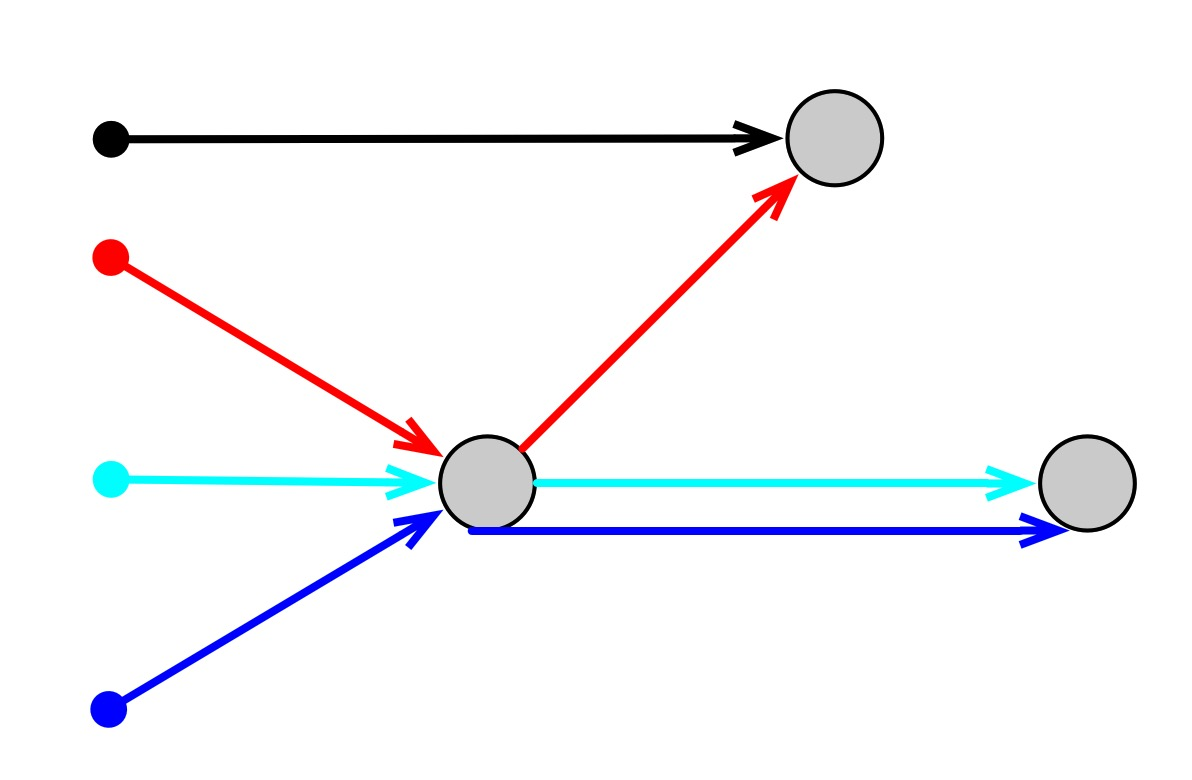
\includegraphics[width=0.4\textwidth, fbox]{construct-1}
        \label{fig:construct-1}}
    \subfloat[会话位置确定,线条排序]{
        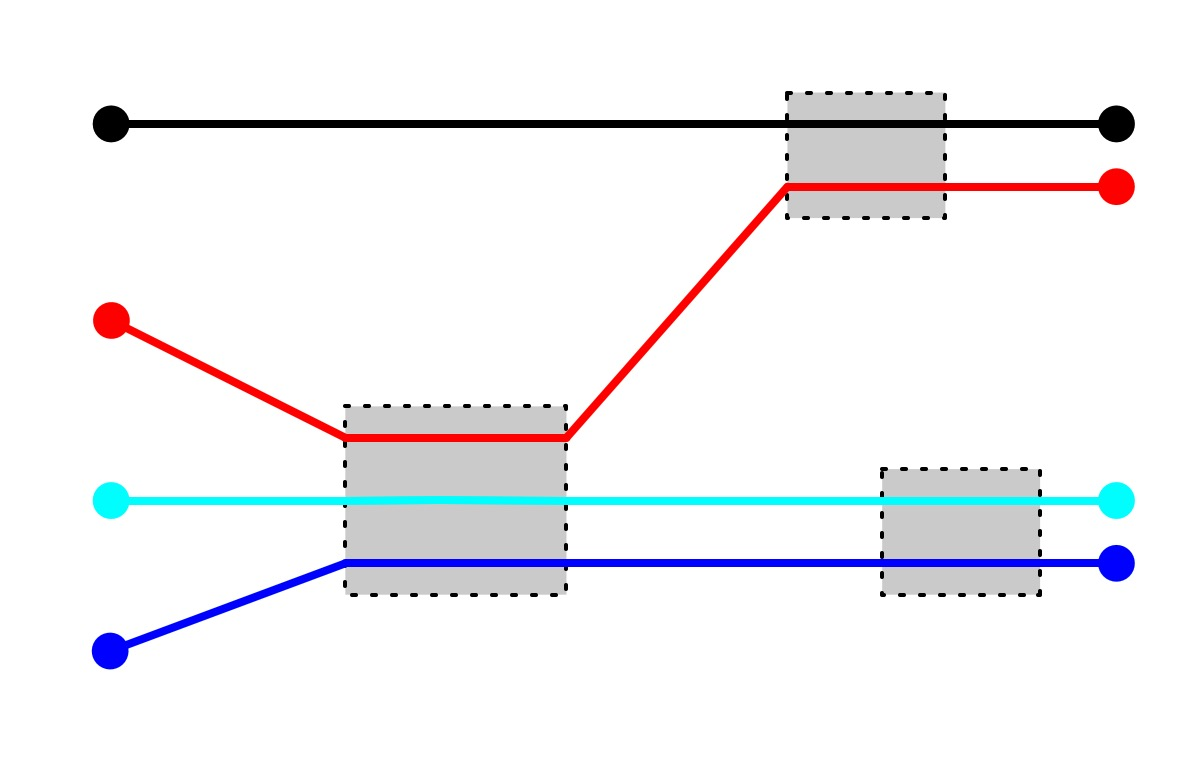
\includegraphics[width=0.4\textwidth, fbox]{construct-2}
        \label{fig:construct-2}}
    \caption{Stroyline 布局方法}
    \label{fig:Storyline-dag}
\end{figure}
%% BEGIN == Construct

布局设计中我们的主要目标就是最小化 \ref{metrics} 小节中提出的三个度量指标:线条交叉,线条摆动和空白距离。 显然这是一个解空间极大的优化问题,要设计一个方法能够同时最优化以上三个指标是一项很困难的任务。对于此类解空间太大而不能轻易求得全局最优解的问题,我们也可以采用遗传算法\cite{tanahashi2012design} 等启发式算法来求得一个接近最优的解决方案。然而,遗传算法的不足是获得的局部最优解经常会比较差,并且容易造成早熟收敛的问题。

既然一步到位同时优化以上三个指标比较困难,很自然的就想到将其分解成几个独立的子问题。每个子问题分别最优化 \ref{metrics} 小节中的一个度量指标。子问题处理的原则是重要指标优先处理,因为它们对最终的可视化效果影响最为严重,更重要的是,在优化后续指标时不能影响前一指标的效果。显然线条交叉对结果的影响,减少线条的摆动以及空白距离次之。基于此,我们将问题分解成以下四个步骤,如图 \ref{fig:layout-steps} 所示:
%% BEGIN == Framework
\begin{figure}[htb]
    \centering
    \subfloat[初始布局]{
        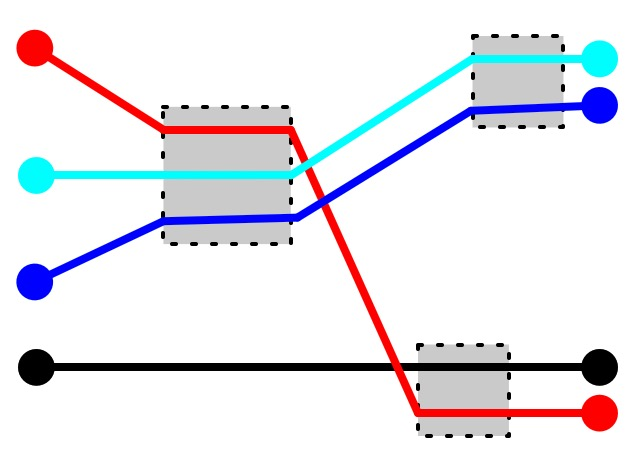
\includegraphics[width=0.22\textwidth, fbox]{framework-1}
        \label{fig:layout-step-1}}
    \subfloat[排序]{
        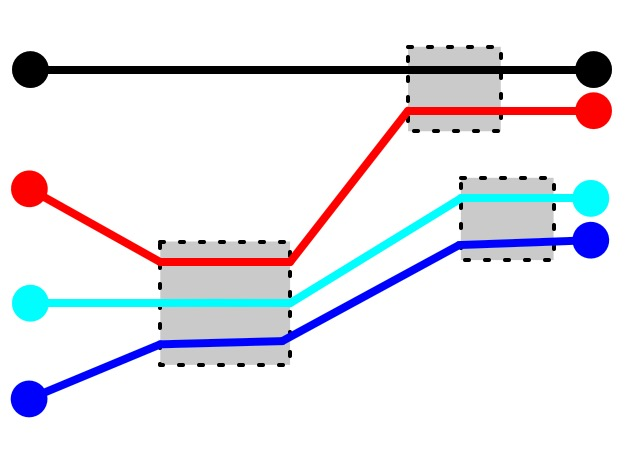
\includegraphics[width=0.22\textwidth, fbox]{framework-2}
        \label{fig:layout-step-2}}
    \subfloat[对齐]{
        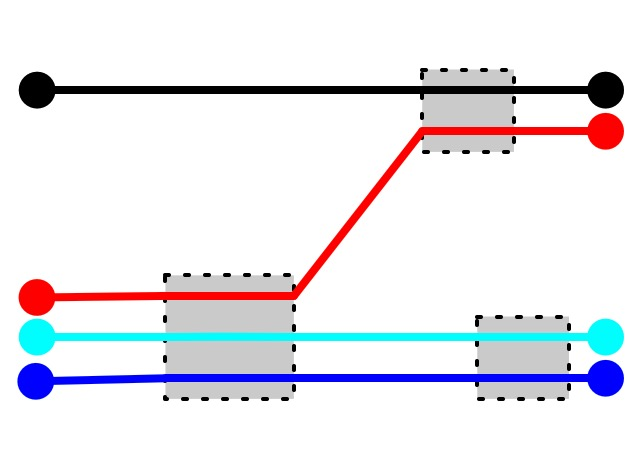
\includegraphics[width=0.22\textwidth, fbox]{framework-3}
        \label{fig:layout-step-3}}
    \subfloat[压缩]{
        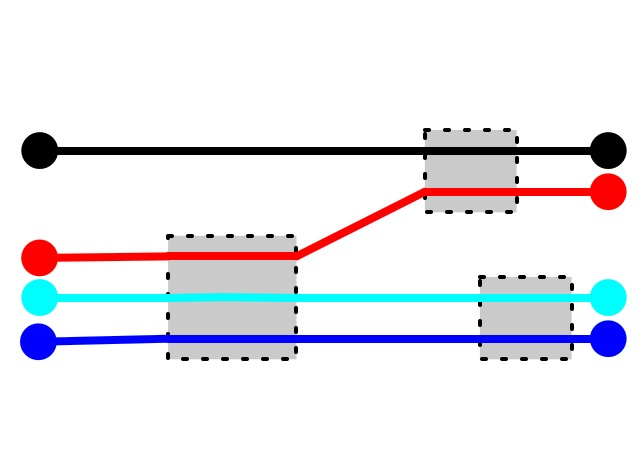
\includegraphics[width=0.22\textwidth, fbox]{framework-4}
        \label{fig:layout-step-4}}
    \caption{布局算法的整体框架}
    \label{fig:layout-steps}
\end{figure}
%% BEGIN == Framework

\begin{asparaenum}[(a)]
\item 初始布局。对于一个优化问题,初始状态对于后面的优化过程往往产生比较重要的影响,一个好的初始状态往往比较容易产生更好的局部最优解。
\item 排序。影响线条交叉数目最直接的因素就是线条的排列顺序,而影响线条排序最重要的因素就是会话的位置,因此为了减少线条不必要的交叉,我们首先要做的就是确定会话的位置。当会话位置确定后,接下来要确定的是会话内部线段的排序,对于同一个代表同一个实体的线条,当会话内部的线段顺序确定后,与该会话相连的线段排序也就相应确定了。
\item 对齐。同样,线条的摆动也直接受会话位置的影响,因此要减少线条的摆动就要在不引入新的交叉的前提下,通过上下微调会话的位置来来使得对齐的线条数量最大化。
\item 压缩。为了使生成的图片更加的美观并且让信息更准确的传递,我们还需要连续的优化空间中的空白距离。
\end{asparaenum}

后面我们将对各个步骤逐一进行进行详细的分析,并提出有效的算法进行求解。

\subsection{初始布局}
正如\ref{section:problem-definition}小节中所描述的,Storyline可以看作是一个DAG图,因此Storyline的初始化过程也是一个DAG图的构建过程。GraphViz\footnote{http://www.graphviz.org/}作为一个经典的图形绘制软件,里面集成了许多优秀的图论和图形绘制算法,dot\cite{Koutsofios1991, Gansner1993a}就是其中之一,dot算法的基本框架如下:
%% BEGIN == DAG构建算法
\begin{algorithm}[htb]
  rank()\;
  ordering()\;
  position()\;
  make\_splines()\;
  \caption{dot算法基本框架}
  \label{algo:draw-graph}
\end{algorithm}
%% END == DAG构建算法
算法第一步rank()的目标是为图中的所有节点分配一个rank,从而使它们分布在不同的rank内;第二步ordering()的目标是分别对每个rank内的节点进行排序,使得排序后的节点产生最少的线条交叉;第三步是为排好序的节点确定坐标值;第四步是绘制连接节点的线条。

dot算法能够很好的绘制出DAG图,但是由于以下原因,它并不能直接用于确定Storyline中节点的位置:
\begin{inparaenum}[\itshape 1 \upshape)]
\item 它将节点作为一个不可细分的单位元素,并且在ordering()时将其视为一个无大小的基本点;而Storyline中每个会话的高度是变化的,参与会话的角色越多,会话的高度就越大;
\item 在DAG图中节点与节点之间一般只有一条边连接,而Storyline中两个会话节点之间一半会有多条边连接;
\item Storyline中节点本身就隐含了rank信息,即可以按会话发生的时间来分配rank。
\end{inparaenum}
尽管如此,我们还是可以通过dot程序来获得会话在垂直方向上的相对位置,并根据它们的相对位置对所有不同rank内的会话进行排序。这样可以获得Storyline内会话的初始排序。

\subsection{排序}
获得会话的初始排序后,后面需要做的就是通过不断调整它们的顺序,使得线条交叉数不断减少。与dot算法中的ordering()步骤不同的是,我们的排序算法由两部分组成:会话(即节点)排序,线段排序。线段排序是指对会话内部表示角色的线条进行排序。
\subsubsection{会话排序}
在会话排序过程中,为了形象的表示会话的顺序,我们将一个平面看成是由一个个水平的slot组成,每个slot的高度由处在该slot内部的会话的高度决定,如图 \ref{fig:order-algorithm} 所示,从上倒下,该图中共有6个slot,并且每个slot内部的会话数量和高度都不尽相同。在实际计算中,slot的个数是随着会话的数量动态调整的。
%% BEGIN == 展示会话详情
\begin{figure}[htb]
    \centering
        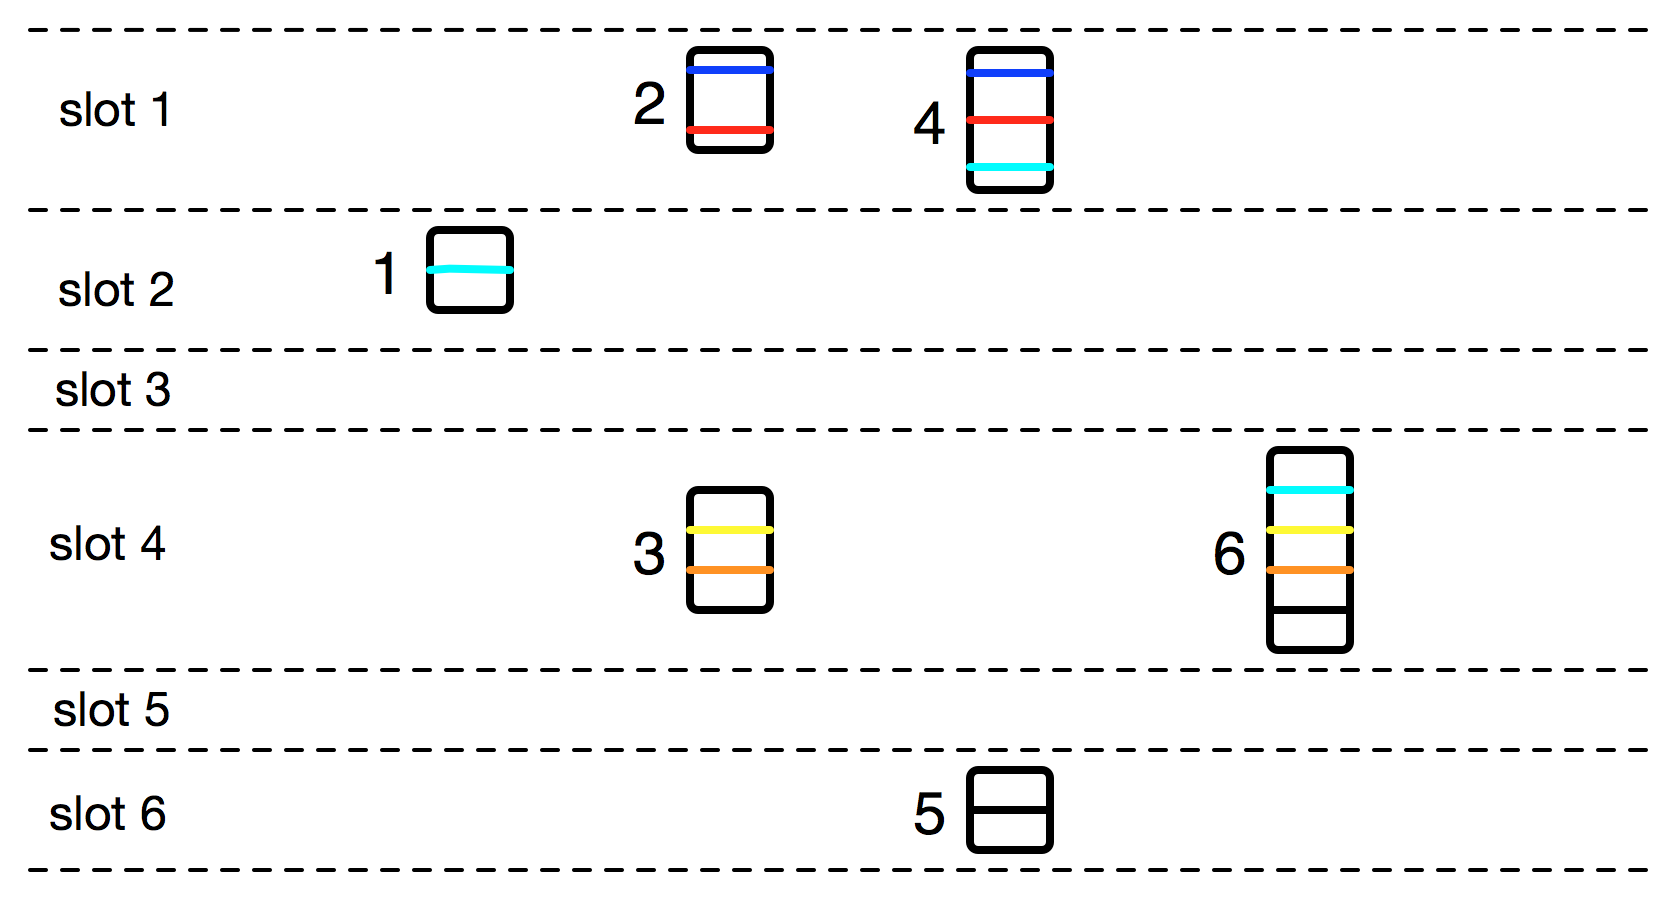
\includegraphics[width=\textwidth, fbox]{order-algorithm}
    \caption{会话排序示意图}
    \label{fig:order-algorithm}
\end{figure}
%% END == 展示会话详情
同一个rank内部的会话顺序,直接决定了线条交叉的数量,好的排序就是要使得交叉数目最少。会话位置调整的基本思想是\cite{warfield1977crossing}:为rank内部的每个会话节点分配一个权重,然后根据权重调将会话放置到各个slot。权重是根据会话的入射点在先前的rank中的位置计算而来。假设$s$表示一个会话,$P$表示与会话$s$相连的入射点的位置列表,那么会话节点$s$的权重等于列表$P$中中位数的值,如果列表$P$中有偶数个元素,那么选取使得线条交叉数少的一个。以图 \ref{fig:order-algorithm}为例,图中4号会话节点中共有三个角色参与(每种颜色的线条分别代表一种角色),红色线条是与4号会话相连的所有入射点集合中的中位数,它在前一个rank中是在slot 1中,因此4号会话的权重也为1,因此被分配在slot 1中。

%% BEGIN == 会话排序算法
\begin{algorithm}[!htb]
  $order = init\_order$\;
  $best = order$\;
  $slots = init\_slots$\;
  \For{$i \leftarrow 1$ \KwTo $max\_iterations$}{
    \For{$r \leftarrow 1$ \KwTo $max\_ranks$}{
      \For{each session $s$ in $order[r]$}{
        $weights[s] = calcWeight(s, r-1)$\;
        $orderSegment(order[r][s])$
      }
      $assignSlots(order[r], weights)$\;
    }
    \For{each slot $t$ in $slots$}{
      $calcHeight(slots[t])$\;
    }
    \If{$crossing(order) < crossing(best)$}{
        $best = order$\;
    }
  }
  \Return best\;
  \caption{会话排序算法}
  \label{algo:session-order}
\end{algorithm}
%% END == 会话排序算法
Algorithm \ref{algo:session-order} 中的$max\_iterations$指最大的迭代次数,该变量的值可以根据多次试验后获得一个经验值,或者通过一个自适应算法,使得线条交叉数目的减少量小于一定比例后才停止迭代。$max\_ranks$指最大的rank值,实验中可以根据数据的时间总跨度自定义每个rank的时间跨度。$order$是一个二维数组,表示所有rank内会话节点的顺序,$order[r]$则表示第$r$个rank内所有会话节点的顺序。
$assignSlots(order[r], weights)$是根据第$r$个rank内会话节点的权重为会话节点重新分配slot。

\subsubsection{线段排序}
会话内部线段排序相对比较简单,它的基本思想是:先根据该线段所表示角色所参与的前一个会话的rank进行排序,如果两个或多个线段所表示的角色同时参与了前一个会话,那么再根据它们在前一个会话内部的顺序进行排序,如Algorithm \ref{algo:line-segment-order}所示。
%% BEGIN == 线段排序算法
\begin{algorithm}[!htb]
  \KwData{line segments in a session}
  \KwResult{line segments in a session after ordering}
  \BlankLine
  $lines = sortByRank(lines)$\;
  $lines = sortByOrder(lines)$\;
  \caption{会话内部线段排序}
  \label{algo:line-segment-order}
\end{algorithm}
%% END == 线段排序算法

\subsection{对齐}
线条对齐主要是为了减少线条的摆动,让更多的线段保持在同一水平直线上,这样有利于读者跟踪角色随时间的变化,避免因线条的交叉和扭动,使得混淆线条与角色的关联关系。通过排序我们已经确定了会话和会话内部线段的相对顺序,但是还没有确定每个元素具体的坐标值。这一小节,我们的目标就是通过确定每个元素具体的坐标值,并且在确定坐标值的时候尽可能的使更多元素保持对齐。

根据上面的分析,我们知道对于会话节点$S$,它的X轴坐标值$X_S$可以根据公式(\ref{eq:x-axis})来确定。
\begin{equation}
\label{eq:x-axis}
X_S = S_{start} * pannel\_width + panel\_shift + session\_sep * (S_{id} -1)
\end{equation}
其中$pannel_width$表示每个单位时间在图形中所表示的像素长度;$panel\_shift$表示整个图形在X轴的水平偏移像素长度;$session\_sep$表示会话之间的固定间隔,目的是为了避免因为会话太多导致图形过于密集。其中$pannel\_width$和$session\_sep$都需要根据具体的实验数据进行调整,对于时间跨度长的数据,$pannel\_width$就需要取相对较小的值;对于会话太多太密集的数据,$session\_sep$就可以取相对较大的值,不然可以直接设为0。这三个参数主要用于控制最重可视化效果,实验中将它们作为参数,方便多次重复实验对比效果。

确定了X轴坐标后,我们需要解决的主要问题是,如何确定会话的Y轴坐标值。在确定Y轴坐标时需要满足几个条件:
\begin{inparaenum}[\itshape 1 \upshape)]
\item 首先需要保证的是会话在垂直方向必须保证一定的间距,用$Min\_V\_Gap$表示;
\item 同在一个会话内部的线段之间的间距$line_sep$,必须要至少小于$Min\_V\_Gap$的一半;
\item 在进行对齐时不能引入新的线条交叉。
\end{inparaenum}
针对每个rank内部会话的Y轴坐标值通过以下的启发式迭代算法进行确定:
%% BEGIN == 对齐算法
\begin{algorithm}[!htb]
  $calcSlotsBound()$\;
  $yaxis = init\_yaxis()$\;
  $ybest = yaxis$\;
  \For{$i \leftarrow 1$ \KwTo $max\_iterations$}{
    $minwiggle(i, yaxis)$\;
    \If{$wiggles(order) < wiggles(ybest)$}{
        $ybest = yaxis$\;
    }
  }
  \Return $ybest$\;
  \caption{对齐算法(确定Y轴坐标值)}
  \label{algo:alignment}
\end{algorithm}
%% END == 对齐算法

Algorithm \ref{algo:alignment}中第一步$calcSlotsBound()$是根据排序过程中获得slot信息,确定每个slot在垂直空间上的上限和下限坐标值,每个slot的宽度必须确保大于该slot内高度最高的一个会话,并且为了给后面的对齐提供足够的空间,尽量使slot的宽度大一些。接着我们要根据排序结果来计算会话和会话内线段的初始坐标,$init\_yaxis()$的对该rank内的所有会话按照所在slot从上往下进行Y轴坐标值初始化,对于slot 1里面的会话,随机赋值,然后根据该会话内的角色数量确定会话的高度;接着初始化后续slot内的会话,对于后续的会话只需在前一个会话的基础上加上$Min\_V\_Gap$值即可。在迭代的过程中,算法的启发因子是,通过向上或向下调整会话的位置,使得连接该rank与前后两个rank的线条尽可能多的保持对齐,也即最小化线段的波动。需要注意的是,上下调整会话位置的过程中,会话不能超过其所在slot的上下限。

\subsection{压缩} 
在排序和对齐过程中,为了保证足够的调整和优化空间,我们在计算slot的界限时刻意保留较大的宽度。因此在压缩过程中,我们首先压缩的空间是重新调整slot的宽度,将slot间多余的空间去掉。
%% BEGIN == 压缩算法
\begin{algorithm}[!htb]
  \For{each slot $i$ in $slots$}{
    $<session_1, tmp_1> = calcSessionMaxY(i)$\;
    $<session_2, tmp_2> = calcSessionMinY(i+1)$\;
    \If{$session_1$ and $session_a$ are not in the same rank}{
      $d = tmp_2 - tmp_1$\;
      $shiftSessionsInSlot(i+1, d)$\;
    }\Else{
      $d = tmp_2 - tmp_1 - Min\_V\_Gap$\;
      $shiftSessionsInSlot(i+1, d)$\;
    } 
  }
  \caption{压缩算法(优化Y轴坐标值)}
  \label{algo:compaction}
\end{algorithm}
%% END == 压缩算法
Algorithm \ref{algo:compaction}依次缩减两两相邻slot的空白间距,首先计算$slot_i$内部所有会话中距离$slot_{i+1}$最近的位置的Y轴坐标值,接着计算$slot_{i+1}$中距离$slot_i$最近的位置的Y轴坐标值,然后计算出它们之间的差值$d$,最后将$slot_{i+1}$中所有会话向上平移$d$。

\section{Storyline 交互式优化}
由上面的分析可以知道,在Storyline的生成过程中,会话位置至关重要,因此在探索Storyline的可交互方面,我们首先考虑的是让用户可以通过拖拽的方式来手动的调整会话的位置,从而达到线条重排序和对齐的效果。其次,由于不同的用户对于信息有不同的偏好和需求,因此我们需要允许用户自己选择需要隐藏或显示的实体。
\subsection{拖拽会话}
通过拖拽重新定位会话的位置,我们可以对已经生成的Storyline进行微调,从而使得最重Storyline更加具表达性且更加的美观。会话在拖拽过程中,该会话内部以及与该会话相连的所有线段都会实时计算新的坐标位置并且进行重绘;会话拖拽结束时,我们需要重新计算所有的会话和所有的线段坐标,并对这个Storyline进行重绘。

拖拽会话最直接的效果就是可以手动调节使得线条对齐,如图 \ref{fig:drag-to-realignment} 所示,通过向下拖拽两个会话使得三个曲线变成了直线。
%% BEGIN == 拖拽会话使对齐
\begin{figure}[htb]
    \centering
    \subfloat[拖拽前]{
        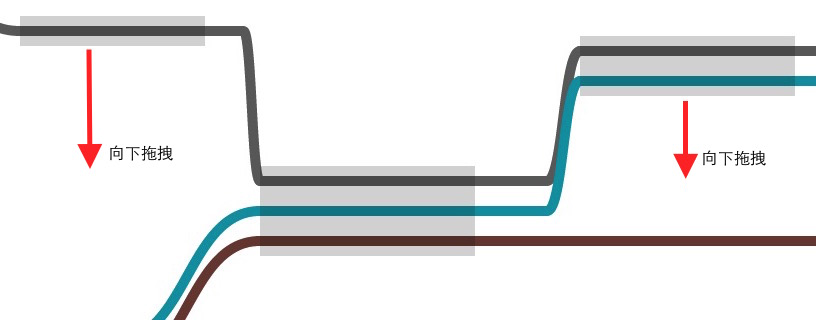
\includegraphics[width=0.4\textwidth, fbox]{alignment-before}
        \label{fig:realignment-before}}
    \subfloat[拖拽后]{
        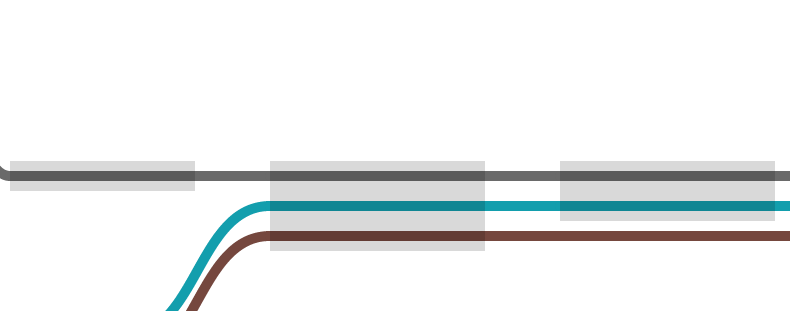
\includegraphics[width=0.4\textwidth, fbox]{alignment-after}
        \label{fig:realignment-after}}
    \caption{通过拖拽会话使得线条对齐}
    \label{fig:drag-to-realignment}
\end{figure}
%% END == 拖拽会话使对齐

通过手动拖拽可以促使线条重新排序,从而减少线条的交叉,如图 \ref{fig:drag-to-reorder} 所示,通过将红色线条的起点拖拽到另外两个线条的小面后,使得线条重新排序,最重减少了两个线条交叉。
%% BEGIN == 拖拽会话使得线条重排序
\begin{figure}[htb]
    \centering
    \subfloat[拖拽前]{
        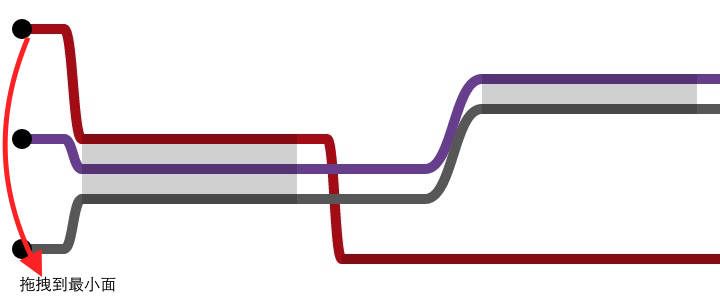
\includegraphics[width=0.4\textwidth, fbox]{order-before}
        \label{fig:order-before}}
    \subfloat[拖拽后]{
        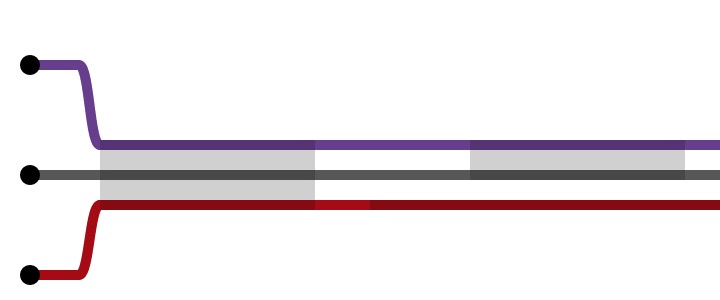
\includegraphics[width=0.4\textwidth, fbox]{order-after}
        \label{fig:order-after}}
    \caption{通过拖拽会话使得线条重排序}
    \label{fig:drag-to-reorder}
\end{figure}
%% BEGIN == 拖拽会话使得线条重排序

\subsection{展示会话详情}
通过Storyline,用户可以了解哪些实体在什么时间点发生了交互,但是却不知道在该时间点它们之间具体发生了什么事情。为了更好的让用户了解每个会话所发生的事件详情,我们为每个会话都添加了上下文信息。当鼠标移动到会话位置,会出现一个弹框,弹框内包含了该会话的主题,以及与该会话相关的文章的链接地址。用户可以通过主题词了解事件的重要信息,同时还可以点击具体的详情文章了解具体信息,如图 \ref{fig:session-with-context} 所示。
%% BEGIN == 展示会话详情
\begin{figure}[htb]
    \centering
        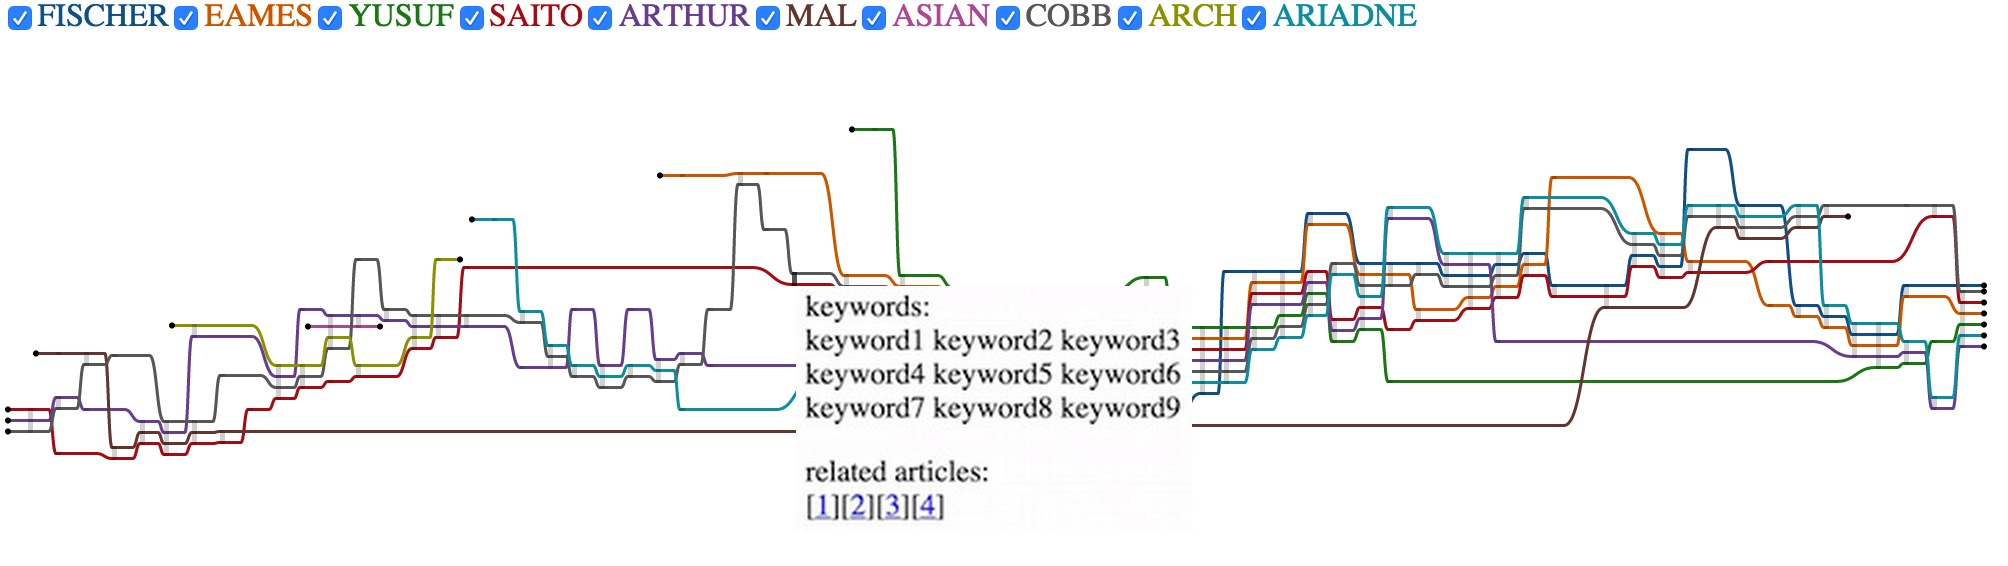
\includegraphics[width=\textwidth, fbox]{session-with-context}
    \caption{显示会话详情}
    \label{fig:session-with-context}
\end{figure}
%% END == 展示会话详情

\subsection{隐藏/显示实体}
在生成的Storyline中,有时实体数量会比较多,因此线条关系会比较复杂。对于某一个用户而言,它并不需要同时查看所有的实体之间的关系,因此允许用户隐藏他不关心的实体,仅保留他关心的实体显得非常实用。对于隐藏的实体,若用户可以重新勾选使其展现出来。隐藏和显示实体并不影响原始的Storyline布局,因此用户可以随意组合自己想要查看的实体,如图 \ref{fig:hide-character} 所示,其中图 \ref{fig:hide-character-before}为显示所有实体时的效果,图 \ref{fig:hide-character-after}为隐藏部分实体后的效果。
%% BEGIN == 隐藏和显示实体
\begin{figure}[htb]
    \centering
    \subfloat[]{
        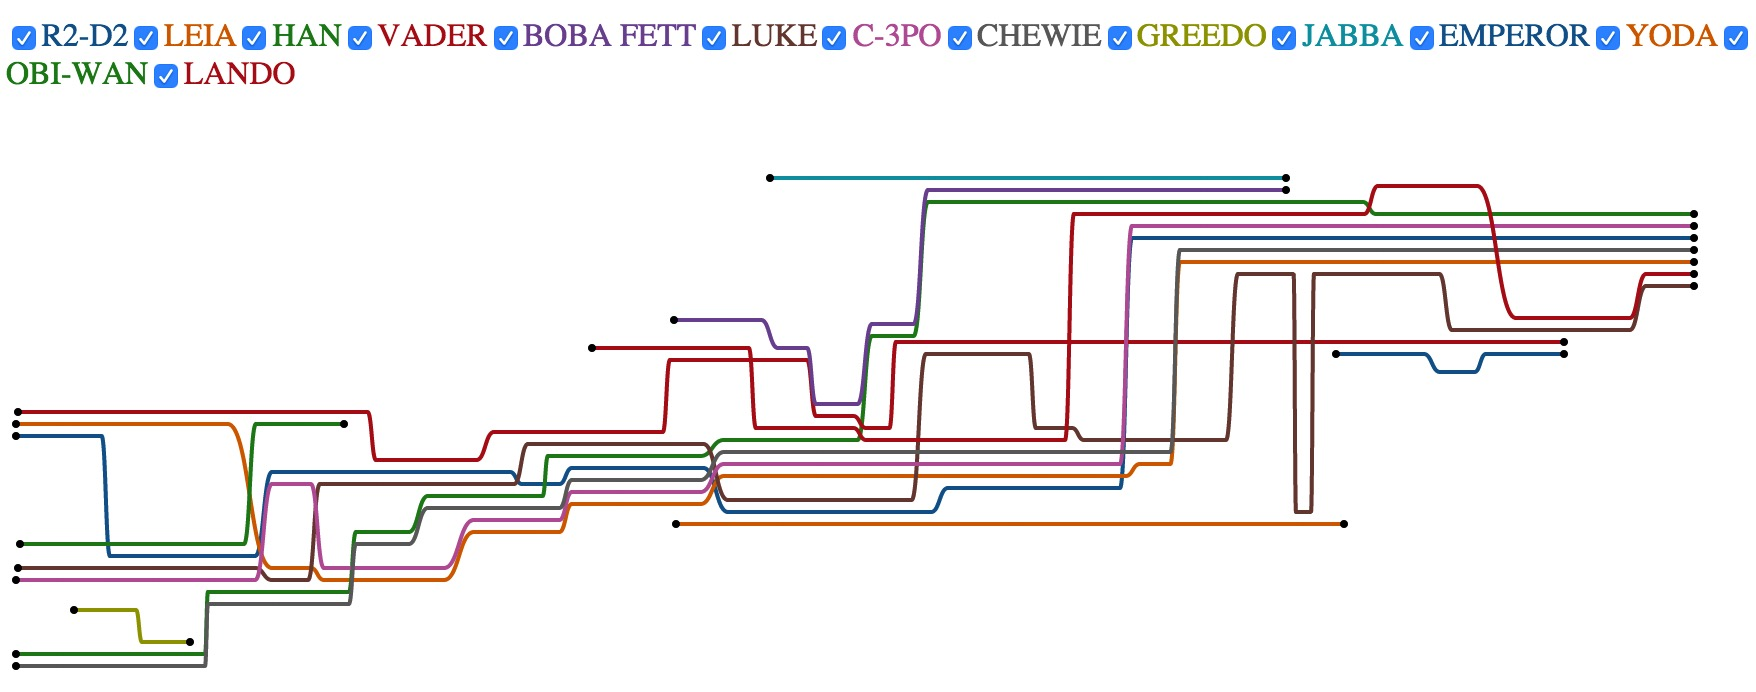
\includegraphics[width=\textwidth, fbox]{hide-character-before}
        \label{fig:hide-character-before}}

    \subfloat[]{
        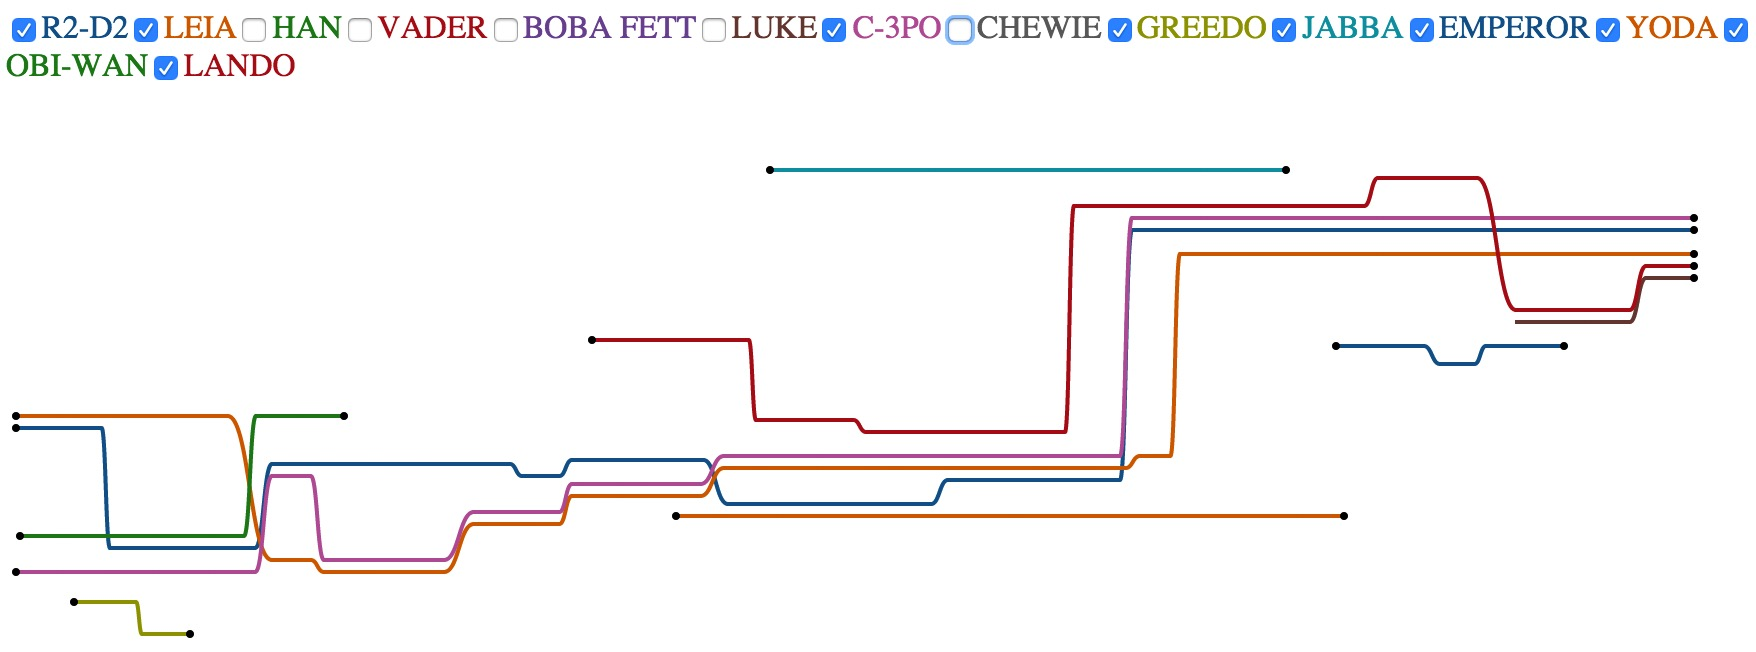
\includegraphics[width=\textwidth, fbox]{hide-character-after}
        \label{fig:hide-character-after}}
    \caption{显示和隐藏实体}
    \label{fig:hide-character}
\end{figure}
%% BEGIN == 隐藏和显示实体

\section{可视化实现}
为了更好的展示可视化结果并提供交互式的用户体验,我们选择了Web端作为展示平台,因此在实现过程中使用的主要技术为JavaScript和SVG,并且使用了d3.js\footnote{http://d3js.org/},Viz.js\footnote{https://github.com/mdaines/viz.js}和Graphlib-dot\footnote{https://github.com/cpettitt/graphlib-dot/wiki}等开源框架来来帮助我们实现绘图以及运行和解析DOT文件。
\subsection*{线条绘制}
在Storyline中主要包括两类线段,分别是:会话内部的线段,连接会话的线段。对于会话内部的线段,在绘图是我们只需将其保持水平即可,也就是只需要线段的起点和终点坐标就可以确定。然而对于连接两个会话的线段,如果仅仅是用直线将其连接起来,会使Storyline中出现趋多折线,看起来不够平滑。因此连接会话的线段我们需要用曲线去表示,在SVG中可以使用贝塞尔曲线\footnote{http://en.wikipedia.org/wiki/Bezier\_curve}来表示Path。我们采用三次曲线,它由两个端点$a$,$b$以及两个中介点$m1$,$m2$来确定,通过实验分析,我们最终选择了如图 \ref{fig:bezier-curve} 所示的中介点来控制曲线。中介点的坐标根据公式(\ref{eq:align})确定。
\begin{subequations}
\label{eq:align}
\begin{align}
    x_{m1} = \frac{1}{2}\left ( x_a + x_b \right ), \quad y_{m1} = y_a \\
    x_{m2} = \frac{1}{2}\left ( x_a + x_b \right ), \quad y_{m2} = y_b
\end{align}
\end{subequations}
为了让连接会话的线段尽可能保持对齐,我们不能简单的将线段的起点和终点作为曲线的两个端点,而应在线段上靠近终点附近开始绘制曲线,而其余部门则保持水平对齐。对于线段$ab$,曲线起点$s$根据公式(\ref{eq:curve-start})进行选取。
\begin{equation}
\label{eq:curve-start}
x_s = x_b - Min(panel\_width*10, (x_b - x_a)*3.0/10.0);
\end{equation}
其中$pannel\_width$表示每个单位时间所占的像素长度。从公式 (\ref{eq:curve-start}) 可以看出,如果线段的起点和终点在水平方向上相距较远,则曲线的起点设置成距离终点10个单位时间的长度;相反如果它们距离很近,则设置为距离终点$3/10$的地方。以上的具体数值是根据实验分析得到的经验值,可以根据实际情况进行调整。
%% BEGIN == segment
\begin{figure}[htb]
    \centering
    \subfloat[三次曲线中介点选取]{
        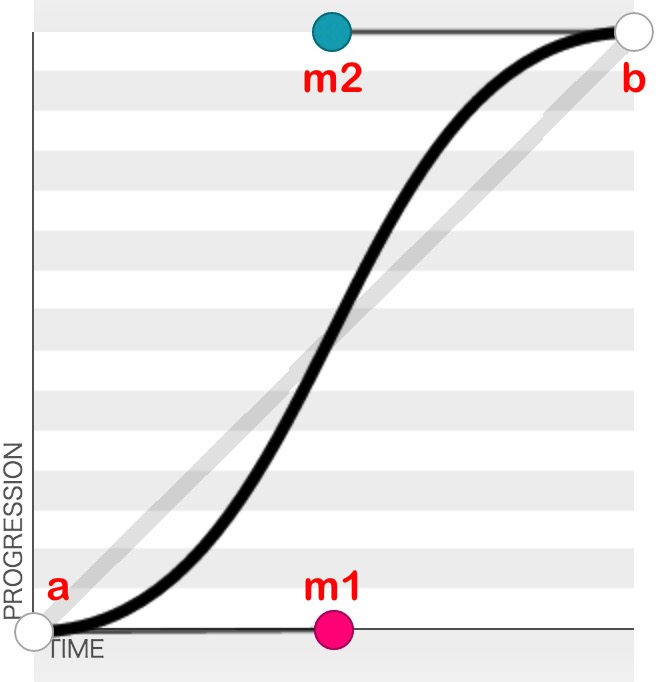
\includegraphics[width=0.27\textwidth, fbox]{bezier-curve-sample}
        \label{fig:bezier-curve}}
    \subfloat[曲线实例1]{
        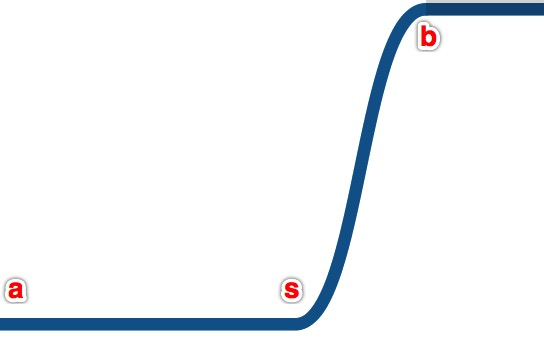
\includegraphics[width=0.45\textwidth, fbox]{bezier-curve-instance1}
        \label{fig:bezier-curve-instance1}}
    \subfloat[曲线实例2]{
        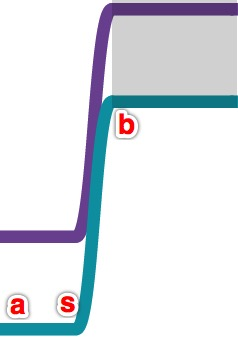
\includegraphics[width=0.195\textwidth, fbox]{bezier-curve-instance2}
        \label{fig:bezier-curve-instance2}}
    \caption{会话之间的连接线段绘制}
    \label{fig:session-space}
\end{figure}
%% END == segment

\section{实验结果与分析}
本小节,我们首先通过定量的分析,将本文方法与Tanahashi 和 Ma\cite{tanahashi2012design}方法进行对比。然后采用 Storyline 方法对上一章节中的“Edward Snowden”这一新闻事件进行实体关系分析,让用户可以从实体的角度出发了解事件的发展,以及关键实体对事件的影响。
\subsection{定量分析}
为了验证本文所提出的Storyline生成方法的有效性,我们与Tanahashi 和 Ma\cite{tanahashi2012design}提出的方法进行比较(为了简化,后文用TM来表示他们提出的方法)。实验中,我们采用了三个数据集,数据采集自三部电影,分别是:“Starwars”,“Inception”和“The Matrix”。图 \ref{fig:layout-comparison} 分别展示了使用用本文方法以及TM方法生成的“Inception”和“The Matrix”的Storyline的效果图,其中图 \ref{fig:inception}和\ref{fig:matrix}由本文方法生成,图 \ref{fig:inception-tm}和\ref{fig:matrix-tm}由TM方法生成。
%% BEGIN == 布局效果对比
\begin{figure}[!htb]
    \centering
    \subfloat[]{
        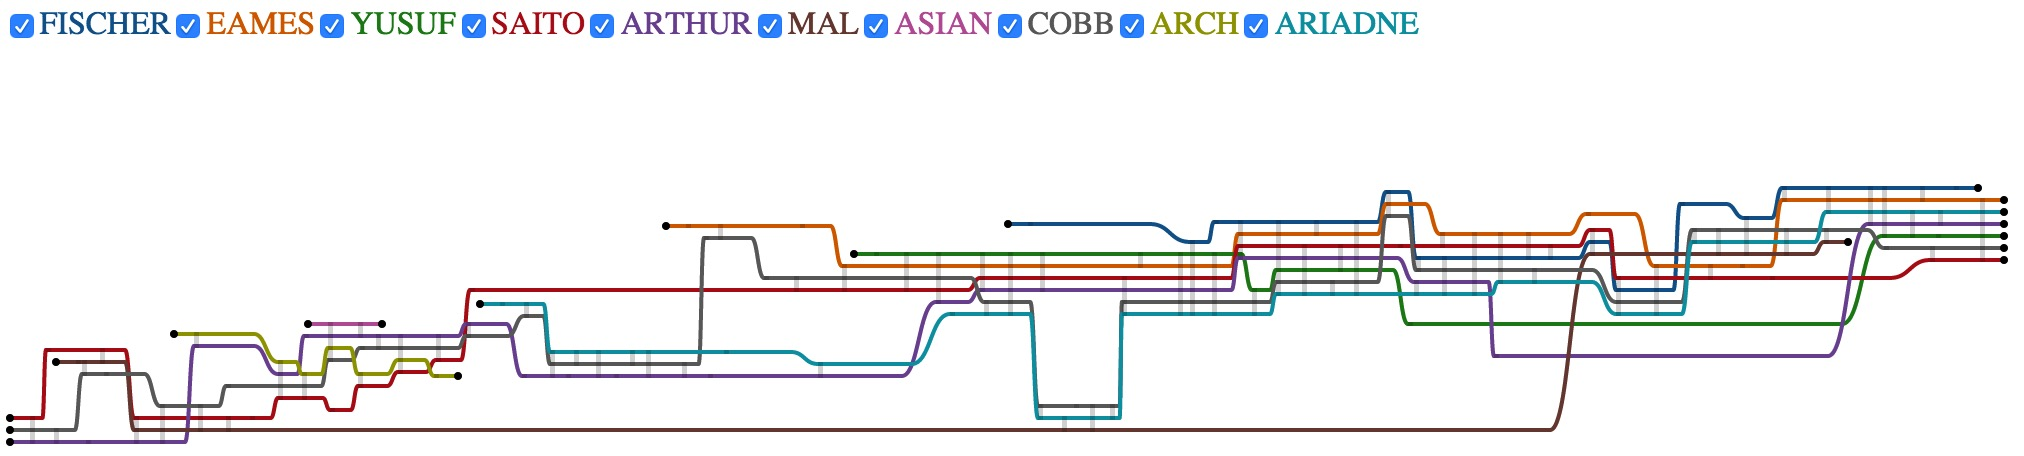
\includegraphics[width=\textwidth, fbox]{layout-inception}
        \label{fig:inception}
    }

    \subfloat[]{
        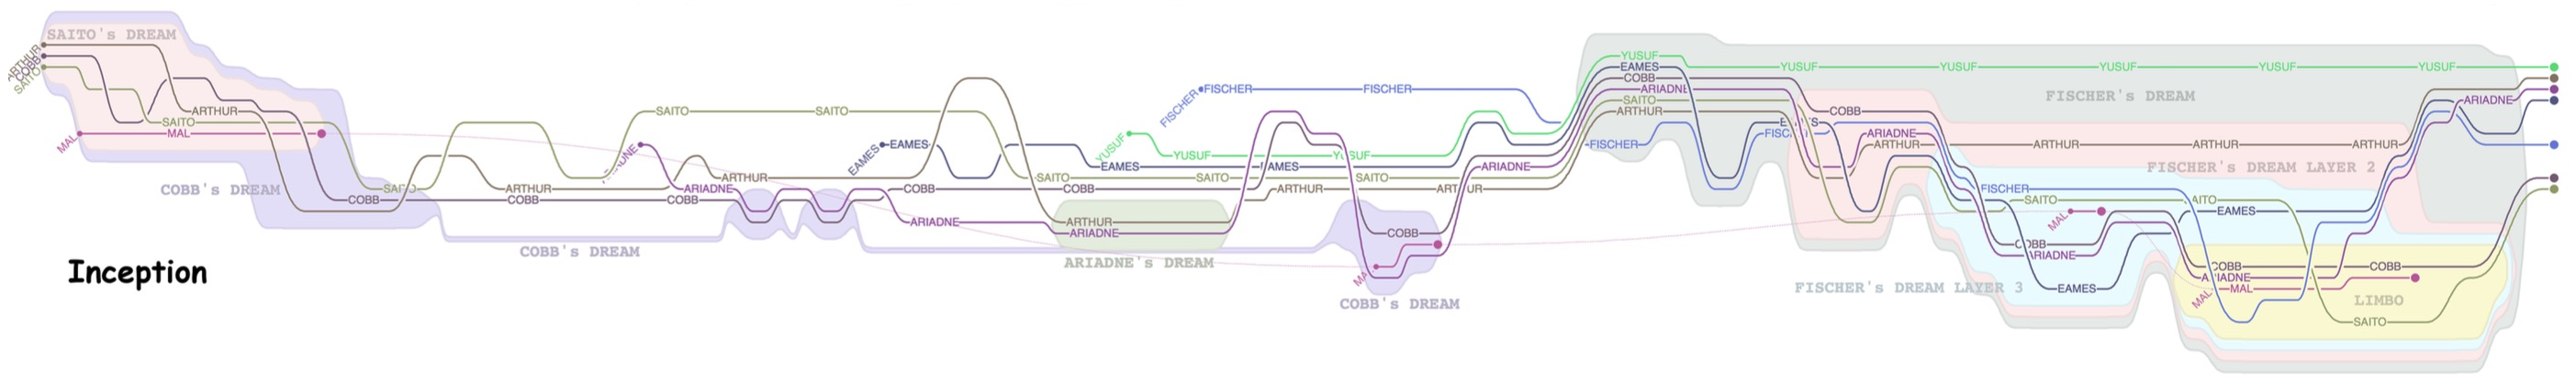
\includegraphics[width=\textwidth, fbox]{layout-inception-tm}
        \label{fig:inception-tm}
    }

    \subfloat[]{
        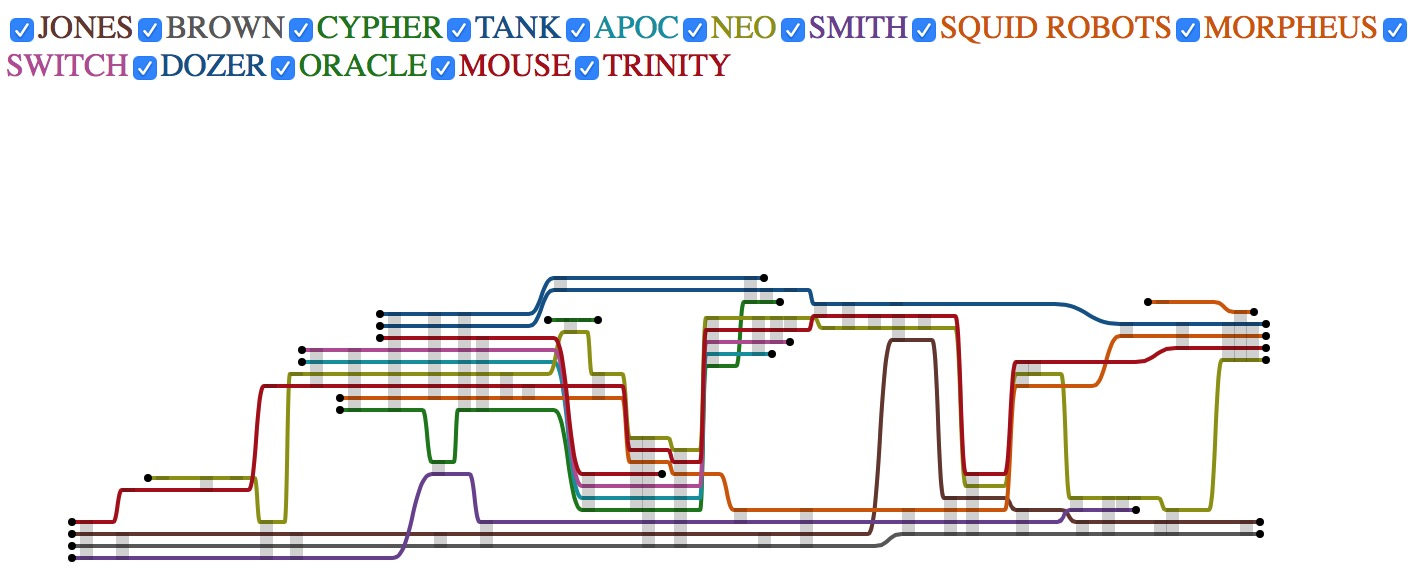
\includegraphics[width=\textwidth, fbox]{layout-matrix}
        \label{fig:matrix}
    }

    \subfloat[]{
        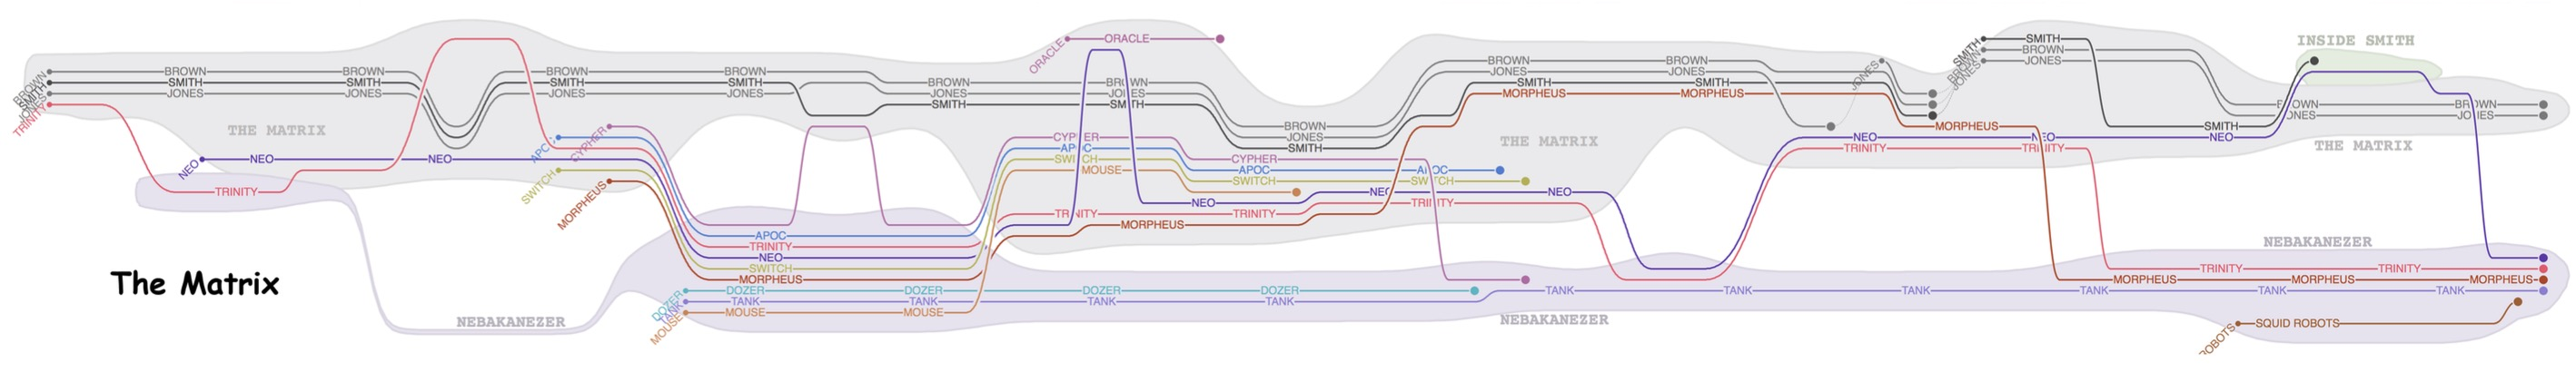
\includegraphics[width=\textwidth, fbox]{layout-matrix-tm}
        \label{fig:matrix-tm}
    }

    \caption{电影 “Inception” 和 “The Matrix” 的 Storyline 效果图对比}
    \label{fig:layout-comparison}
\end{figure}
%% END == 布局效果对比图 
TM方法生成的效果图直接来源于Tanahashi 和 Ma\cite{tanahashi2012design}的论文。两组效果图中,TM方法在图形中添加了位置信息,而本文方法生成的图形中并没有添加这一信息,该信息只是在Storyline的基础上添加的一些辅助信息,对Storyline的生成没有任何影响。在我们生成的Storyline中,我们添加了会话信息(用阴影矩形框表示)。

实验中,我们比较三个指标:运行时间,线条交叉数和线条摆动数。TM方法所产生的实验结果是根据他们的网站上\footnote{http://vis.cs.ucdavis.edu/~tanahashi/data\_downloads/Storyline\_visualizations/}提供的源码运行所得,由于遗传算法每次的结果均不完全一样,因此表 \ref{table:quantitative-analysis} 中的数据是10次试验所得的平均值。

%% BEGIN == 实验结果对比表
\begin{table}[!htb]
\caption{本文方法与TM方法的定量对比}
\label{table:quantitative-analysis}
\begin{center}
  \begin{tabular}{|*{9}{l |}}
    \hline
              & \multicolumn{2}{c|}{数据源} & \multicolumn{2}{c|}{运行时间(秒)} & \multicolumn{2}{c|}{线条交叉数} & \multicolumn{2}{c|}{线条摆动数} \\
    \hline
              & 实体数  & 会话数  & 本方法  & TM方法  & 本方法  & TM方法  & 本方法  & TM方法 \\ \hline
    StarWars  & 14     & 65     & 3     & 141    &  48    &  73    &  66    & 98    \\ \hline
    Inception &  8     & 96     & 3     & 178    &  49    &  97    &  82    & 149   \\ \hline
    Matrix    & 14     & 39     & 3     & 217    &  26    &  43    &  50    & 91    \\ \hline
  \end{tabular}
\end{center}
\end{table}
%% END == 实验结果对比表

从表 \ref{table:quantitative-analysis} 可以很清楚的看到,TM方法所消耗的时间是本文方法的几十倍以上。原因是TM算法是基于遗传算法进行优化,而遗传算法的问题之一就是它需要设置一个较大的繁衍代数,因此消耗的时间会很长。同样,本文方法在减少线条交叉数目以及线条摆动方法也表现更加优秀,因为遗传算法的另一个缺点是,容易陷入局部最优。而本文首先通过构架一个 DAG 图获得了一个较优的初始布局,然后通过后面的迭代算法,能够在较短时间内找到一个更好的局部最优解。

\subsection{案例分析}
本小节用Storyline来分析新闻事件中实体的交互关系,并以“Edward Snowden”事件为例。为了生成Storyline,首先我们要从文档集合生成列表 \ref{list:json-sample} 所示的输入数据,输入数据的生成过程包括以下几个步骤,如图 \ref{fig:case-analysis-framework} 所示。

%% BEGIN == 命名实体抽取
\begin{figure}[htb]
    \centering
        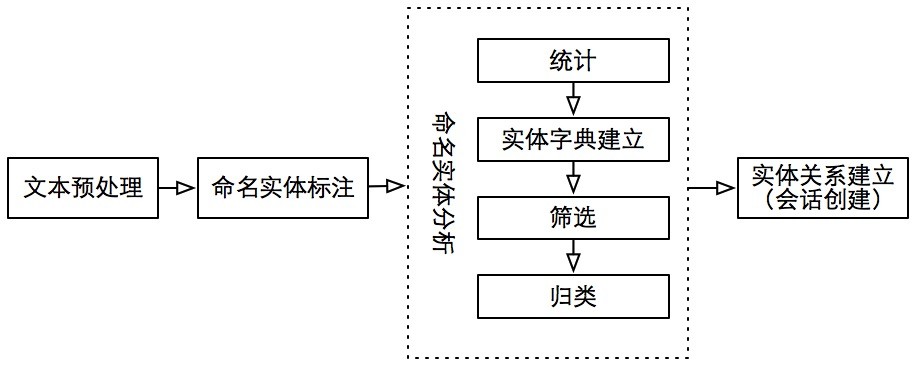
\includegraphics[width=0.8\textwidth, fbox]{case-analysis-framework}
    \caption{命名实体自动抽取和会话创建}
    \label{fig:case-analysis-framework}
\end{figure}
%% END == 命名实体抽取

\begin{enumerate}[(1)]
\item 文本预处理,获得文档编号与文档发生日期的映射关系。
\item 命名实体标注,是指将文本中的人名,地名,国家,组织机构等等识别出来并用标签进行标注。本实验中,我们采用 AlchemyAPI\footnote{http://www.alchemyapi.com/} 提供的开放API进行命名实体标注。当我们将所有文档中出现的所有实体(保留了人名,国家和机构)识别出来后,我们用标签云进行实体的可视化后(见图 \ref{fig:entity-cloud}),可以很清楚的看出事件中一些重要的实体信息。
\item 命名实体分析,首先,统计每个实体$E_i$在所有文档中出现的总次数$E_i^n$,总共出现在多少文档当中$E_i^d$;其次,建立命名实体词典,为每个实体分配编号;接着,对命名实体进行筛选,仅保留出现符合条件的实体(本实验中,筛选条件为:$E_i^n > 100$ 且 $E_i^d > 100$);最后对保留下来的实体进行归类整理,获得每个实体对应的文档编号列表$Docs_i$(按文档产生的时间顺序从小到大排序),该列表表示这个实体在这些文档中出现过。
\item 会话创建,是指建立命名实体之间的交互关系。本实验中,我们假定两个实体如果在同一片文章或在同一天的不同文章中一起出现,则认为他们之间发生了交互。因此,我们首先需要将上一步中获得的$Docs_i$中的文档编号映射到日期上,获得每个实体对应出现的日期列表$Dates_i$;然后根据$Dates_i$的集合创建出实体之间交互的会话列表。
\end{enumerate}
%% BEGIN == Edward Snowden Entity Cloud
\begin{figure}[htb]
    \centering
        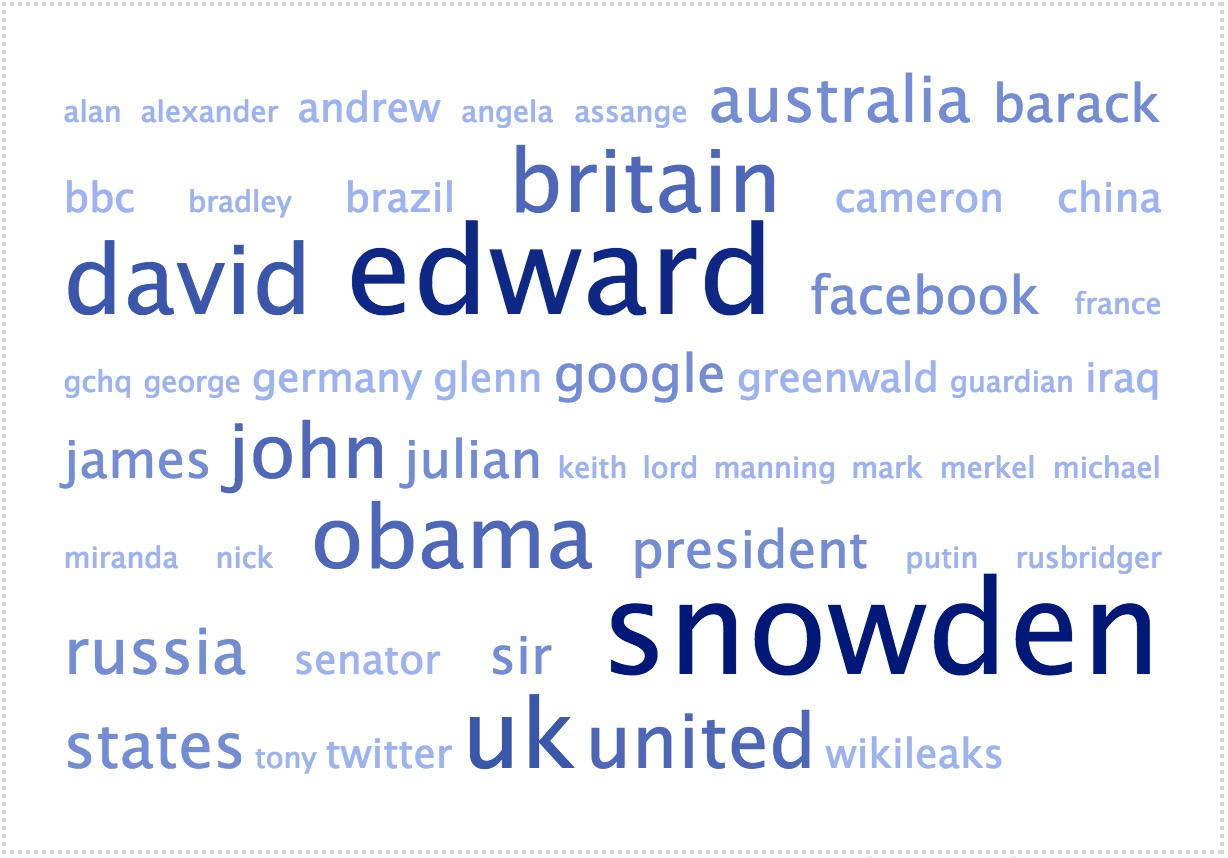
\includegraphics[width=0.6\textwidth, fbox]{entity-cloud}
    \caption{"Edward Snowden" 事件相关实体云}
    \label{fig:entity-cloud}
\end{figure}
%% END == Edward Snowden Entity Cloud

通过以上预处理获得Storyline的输入数据后,通过Storyline的生成算法可以创建出如图 \ref{fig:case-snowden-layout} 所示的图形。
%% BEGIN == Edward Snowden Storyline Layout
\begin{figure}[htb]
    \centering
        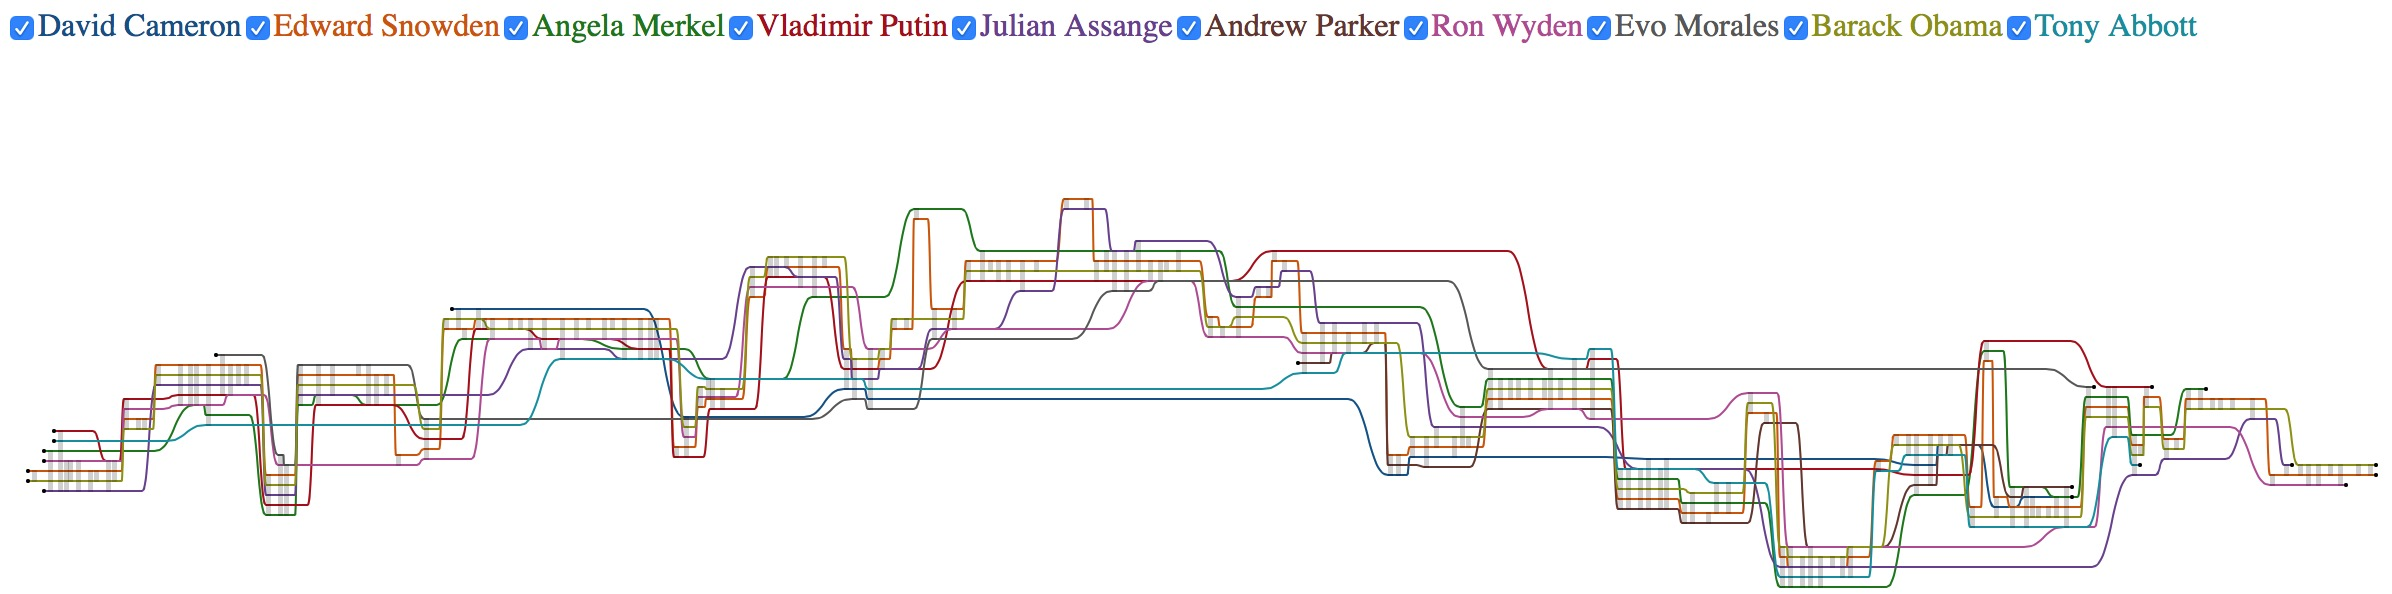
\includegraphics[width=\textwidth, fbox]{case-snowden-layout}
    \caption{"Edward Snowden" 事件关键人物交互关系图}
    \label{fig:case-snowden-layout}
\end{figure}
%% END == Edward Snowden Storyline Layout
从图中我们可以看到,该事件的最核心的人物包括了Obama,Putin,Cameron,Merkel等,分别代表了与该事件相关的各个核心国家。由于我们在会话定义时,认为两个实体在同一篇文章或同一天中出现过即认为他们在一个会话中,因此上图中会话比较密集,并且每个会话内的实体比较多,进而影响了最终的可视化效果。在未来的工作中,我们可以通过更加严谨的方法来抽取会话,进而获得更好的Storyline。
\section{本章小结}
本章我们首先介绍了一种可视化方法-Storyline,该方法是用于描述实体之间随时间变化的交互关系。然而已有的生成Storyline 的方法中,有些是针对特定领域的,有些是计算过程非常耗时的,有些需要纯手动绘制。为了能运用Storyline来描述新闻事件中人物之间的交互关系,我们提出了自己的一套方法来生成Storyline。该方法分三个步骤:排序,对齐,压缩。每一步分别对Storyline的一个指标进行优化,通过迭代的方法最终获得一个最优的图形。最后,我们还根据Storyline的特点提供了几种用户交互方式,既可以进一步优化图形,还可以让用户更好的理解事件详情。
